\chapter{引力波基础}\label{chap:gwbasis}

在本章中,我们将回顾引力波的基础知识,包括引力波的传播方程的推导、引力波的能动张量的定义、标量诱导引力波的计算以及脉冲星计时阵列探测随机引力波背景的原理。

\section{线性爱因斯坦方程}
我们知道时空几何与物质的关系由爱因斯坦方程描述
\e
G_{\mu \nu} = 8 \pi G T_{\mu \nu},
\q 
其中$G$为牛顿引力常数,$T_{\mu \nu}$是物质场的能动张量在这里。在这里,我们选取光速$c=1$。时空几何由爱因斯坦张量$G_{\mu\nu}$给出,其定义为
\e\label{einstein}
G_{\mu\nu} \equiv R_{\mu\nu} - \hf R g_{\mu\nu},
\q 
其中$R_{\mu\nu}$为里奇张量。由于引力耦合常数$G$很小,所以由于引力辐射而产生的引力波非常微弱。在弱场近似下,度规$g_{\mu\nu}$可以分解为闵氏度规$\eta_{\mu\nu}$及其微扰$h_{\mu \nu}$,即
\e 
g_{\mu\nu} = \eta_{\mu\nu} + h_{\mu \nu},\quad |h_{\mu \nu}| \ll 1.
\q 
由于$h_{\mu \nu}$是个小量,所以逆度规可分解为
\e 
g^{\mu\nu} = \eta^{\mu\nu} - h^{\mu \nu}.
\q
进而可以算出联络的为
\m 
\ts{\Ga}{^\la_\mu_\nu} &\equiv& \hf g^{\la\sg} \( \p_\mu g_{\nu\sg} 
+ \p_\nu g_{\mu\sg} - \p_\sg g_{\mu\nu} \) \\
&=& \hf \( \p_\mu \Th{_\nu^\la}
+ \p_\nu \Th{_\mu^\la} - \p^\la h_{\mu\nu} \).
\n
由上式可知联络是微扰$h_{\mu \nu}$的一阶小量,所以只有联络点一阶导数对里奇张量有贡献,即
\m\label{ricci}
R_{\mu \nu} &=& \p_\al \TG{^\al_\mu_\nu} - \p_\nu \TG{^\al_\mu_\al} \\
&=& \hf \( \p_\al \p_\mu \Th{_\nu^\al}
+ \p_\al \p_\nu \Th{_\mu^\al} - \DA h_{\mu\nu} 
- \p_\mu \p_\nu h \).  
\n
上式中的$\DA$为达朗贝尔算符,其定义为
\e 
\DA h_{\mu\nu} \equiv \p_\al \p^\al h_{\mu\nu}.
\q 
同时,里奇标量为
\e 
R = \p_\mu \p_\nu h^{\mu \nu} - \DA h.
\q 
利用\eqref{einstein}式,可算出爱因斯坦张量为
\e
G_{\mu\nu} = \hf\(\p_\sigma \p_\nu \Th{^\sigma_\mu} + \p_\sigma\p_\mu\Th{^\sigma_\nu} - \p_\mu \p_\nu h - \DA h_{\mu\nu} - \eta_{\mu\nu} \p_\al\p_\la h^{\al\la} + \eta_{\mu\nu} \DA h\).
\q 
下面引入迹相反的扰动$\bar{h}_{\mu \nu}$,其定义为
\e
\bar{h}_{\mu \nu} \equiv h_{\mu \nu} - \hf h \eta_{\mu \nu}.
\q 
注意$\bar{h}_{\mu \nu}$和$h_{\mu \nu}$的迹是相反的,即
\e
\bar{h} = \eta^{\mu \nu} \bar{h}_{\mu \nu} = -h.
\q 
下面我们选取洛仑兹规范,即要求$\bar{h}^{\mu \nu}$是横向的,使得
\e 
\p_\mu \bar{h}^{\mu \nu} = 0.
\q 
需要注意的是原始的扰动$h_{\mu\nu}$并不是横向的,因为其满足
\e 
    \p_\mu h^{\mu\nu} = \hf \p^\nu h.
\q 
在洛仑兹规范下,爱因斯坦张量为
\e 
G_{\mu\nu} = - \hf \DA \bar{h}_{\mu\nu}.
\q 
所以在洛仑兹规范下,线性爱因斯坦方程是波动方程,即
\e 
\DA \bar{h}_{\mu\nu} = -16 \pi G T_{\mu \nu}.
\q 
上式可以用来计算线性理论下的引力波的产生。为了考虑引力波的传播以及引力波对探测器的响应,我们需要考虑波源之外的引力波方程,即$ T_{\mu \nu}=0$,进而有
\e\label{propGW}
\DA \bar{h}_{\mu\nu} = 0.
\q
上式表明引力波是以光速传播的。上式还有多余的自由度,在考虑引力波传播的时候,通常选取横向无迹(transverse-traceless,简称TT)规范,即要求
\e 
\p^\mu h^{\TTT}_{\mu \nu} = 0, \quad h^{\TTT} = 0.
\q 
\section{引力波的能动张量}
由于引力是非定域的,所以我们无法毫无争议地给出引力场能量的局部定义。在弱场近似下,由于背景是平坦的闵氏时空,所以我们有可能给出引力波能动张量的定义。我们知道引力波的能量是二阶效应,所以需要对度规展开到二阶,即
\begin{equation}
    \label{eq:GRb_gExp}
    g_{\alpha \beta} = \eta_{\alpha \beta} + h^{\tiny (1)}_{\alpha \beta} + h^{\tiny (2)}_{\alpha \beta}\,,
\end{equation}
其中$h^{\tiny (1)}_{\alpha \beta}$和$h^{\tiny (2)}_{\alpha \beta}$分别为度规的一阶和二阶扰动。有了度规扰动,我们可以将爱因斯坦方程展开到二阶。$h^{\tiny (1)}_{\alpha \beta}$要满足线性阶的扰动方程,即
\begin{equation}
    \label{eq:GRb_FE-order1}
    G_{\alpha \beta}[h^{\tiny (1)}] = 0\,.
\end{equation}
将爱因斯坦方程展开到二阶可以得到
\begin{equation}
    \label{eq:GRb_FE-order2}
    G_{\alpha \beta}\left[h^{\tiny (2)}\right] = 8 \pi G \Theta_{\alpha \beta} \equiv - \left<G_{\alpha \beta}\left[\left(h^{\tiny (1)}\right)^{2}\right]\right> \,.
\end{equation}
上式中的括号$\left< \right>$表示短波平均\cite{Isaacson:1967zz,Isaacson:1968zza}。我们用$\Theta_{\alpha \beta}$表示引力波的能动张量。上式表明一阶扰动产生的能动张量可以作为二阶扰动的源。

我们先考虑场方程的一阶扰动。将里奇张量展开到一阶,其表达式为
\begin{equation}
    \label{eq:GRb_Ricci1o}
    R^{\tiny (1)}_{\alpha \beta}=\frac{1}{2}\left[2\partial_\gamma \partial_{(\alpha}{h_{\beta)}^{(1)\gamma}} - \partial_\alpha \partial_\beta h^{(1)} - \partial_\gamma \partial^\gamma h^{(1)}_{\alpha \beta}\right]\,.
\end{equation}
将上式代入爱因斯坦方程\eqref{eq:GRb_FE-order1}可得
\begin{multline}
    \label{eq:GRb_FE_Exp1o}
    \partial_\gamma \partial_{(\alpha}{h^{\tiny (1)}_{\beta)}}^\gamma - \frac{1}{2}\partial_\alpha \partial_\beta h^{\tiny (1)} - \frac{1}{2}\partial_\gamma \partial^\gamma h^{\tiny (1)}_{\alpha \beta}
    +\frac{1}{2}\eta_{\alpha \beta}\left(\partial_\gamma \partial^\gamma h^{\tiny (1)} - \partial^\gamma \partial^\delta h^{\tiny (1)}_{\gamma \delta}\right)=0 \,.
\end{multline}
在TT规范下,上式可化简得到\Eq{propGW},即
\begin{equation}
    \label{eq:GRb_TTEoM}
    \DA h^{\tiny (1)\TT}_{\alpha \beta}=0\,.
\end{equation}


接下来考虑场方程的二阶扰动。里奇张量的二阶扰动为
    \begin{align}
        \label{eq:GRb_Ricci2o}
        R^{(2)}_{\alpha \beta}=&\frac{1}{2}\left[2\partial_\gamma \partial_{(\alpha}{h_{\beta)}^{(2)\gamma}} - \partial_\alpha \partial_\beta h^{(2)} - \partial_\gamma \partial^\gamma h^{(2)}_{\alpha \beta}\right] + \frac{1}{2} \partial_\beta \left[h^{(1)\gamma \delta}\left(2\partial_{(\alpha}h^{(1)}_{\gamma)\delta}-\partial_\delta h^{(1)}_{\alpha \gamma}\right)\right] \nonumber\\
        &-\frac{1}{2}\partial_\gamma \left[h^{(1)\gamma \delta}\left(2\partial_{(\alpha}h^{(1)}_{\beta)\delta}-\partial_\delta h^{(1)}_{\alpha \beta}\right)\right]+ \frac{1}{4}\partial_\gamma h^{(1)} \left[2\partial_{(\alpha}h^{(1)\gamma}_{\beta)} - \partial^\gamma h^{(1)}_{\alpha \beta}\right] \nonumber\\
        &-\frac{1}{4}\left[\partial_\alpha h^{(1)\gamma \delta}\partial_\beta h^{(1)}_{\gamma \delta}+2 \partial_\gamma h^{(1)\delta}_{\alpha} \partial_\delta h^{(1)\gamma}_{\beta} - 2\partial_\gamma h^{(1)\delta}_{\alpha} \partial^\gamma h^{(1)}_{\beta \delta}\right] \,.
    \end{align}
在TT规范下,上式可化简为
\begin{align}
    \label{eq:GRb_Ricci2}
    R^{(2)}_{\alpha \beta} =& -\frac{1}{2} \partial_\gamma \partial^\gamma h^{(2)\TT}_{\alpha \beta}
    + \frac{1}{4} \partial_\alpha h^{\tiny (1) \gamma \delta}_{\TT} \partial_\beta h^{\tiny (1)\TT}_{\gamma \delta} + \frac{1}{2}h^{\tiny (1)\gamma \delta}_\TT \partial_\alpha \partial_\beta h^{\tiny (1)\TT}_{\gamma \delta} + \frac{1}{2}h^{\tiny (1)\gamma \delta}_\TT \partial_\gamma \partial_\delta h^{\tiny (1)\TT}_{\alpha \beta} \nonumber \\
    &- h^{\tiny (1)\gamma \delta}_\TT \partial_\delta \partial_{(\alpha}h^{\tiny (1)\TT}_{\beta) \gamma}+ \partial_{[\delta}h_{\gamma]\beta}^{\tiny (1)\TT} \partial^\delta h_{\alpha}^{\tiny (1)\TT \gamma}\,.
\end{align}
利用公式\eqref{eq:GRb_FE-order2}可得到引力波的能动张量为
\begin{equation}
    \Theta_{\alpha \beta} = \frac{1}{32 \pi G} \avg{\partial_\alpha h^{\TT}_{\gamma \delta} \; \partial_\beta h^{\gamma \delta}_{\TT}}\,.
\end{equation}
由此可进一步得到引力波的能量密度
\e\label{rhogw}
\rho_{\GW} \equiv \Theta_{00} =  \frac{1}{32\pi G} \av{\p_0 h_{\rho\sg} \p_0 h^{\rho\sg}} = \frac{1}{32\pi G} \av{\dot{h}_{ij} \dot{h}^{ij}}.
\q

\section{标量诱导引力波}
下面我们考虑原初标量扰动产生的次生引力波。在牛顿规范下,扰动的FRW(Friedmann-Robertson-Walker)度规为\cite{Ananda:2006af}
\e
\rd s^{2}=a^{2}\left\{-(1+2 \phi) \rd \eta^{2}+\left[(1-2 \phi) \delta_{i j}+\frac{h_{i j}}{2}\right] \rd x^{i} \rd x^{j}\right\},
\q
其中$\eta$为共形时间,$a$为尺度因子,$\phi \equiv \phi^{(1)}$是标量模式的一阶扰动,$h_{ij} \equiv h_{ij}^{(2)}$为张量模式的二阶扰动。因为我们关心的是由标量扰动$\phi$诱导的引力波$h_{ij}$,所以我们忽略掉矢量扰动。 
在辐射为主时期,通过爱因斯坦方程可以给出傅立叶空间的标量扰动$\phi$的演化方程为
\e
\phi_{\vec{k}}''(\eta)+{4\over\eta}\phi_{\vec{k}}'(\eta)+{k^2\over3}\phi_{\vec{k}}(\eta)=0.
\q
这个运动方程的解为\cite{Baumann:2007zm}, 
\e\label{phi}
\phi_{\vec{k}}(\eta) \equiv \phi_{\vec{k}}\frac{9}{(k\eta)^2} \[  \frac{\sin(k\eta/\sqrt{3})}{k\eta/\sqrt{3}} - \cos(k\eta/\sqrt{3})\],
\q
其中$\phi_{\vec{k}}$是$\eta=0$时的原初扰动,其值由暴胀模型给出。由爱因斯坦方程可以给出二阶张量扰动的运动方程为
\e\label{eqh2}
h_{i j}^{\prime \prime}+2 \mathcal{H} h_{i j}^{\prime}-\nabla^{2} h_{i j}=-4 \mathcal{T}_{i j}^{\ell m} S_{\ell m},
\q
其中一撇表示对共形时间$\eta$的导数,而$\mathcal{H}=a'/a$为共形哈勃参数。上式的源项为\cite{Ananda:2006af}
\e
S_{ij}= 4 \phi \p_i\p_j\phi + 2\p_i\phi\p_j\phi-{1\over\mH^2}\p_i \(\mH\phi + {\phi'}\)\p_j\(\mH\phi + {\phi'}\).
\q
在方程\eqref{eqh2}的右边,我们通过TT投影算符$\mathcal{T}_{i j}^{\ell m}$将源项投影到TT规范下。$\mathcal{T}_{i j}^{\ell m}$的定义为
\e
\mathcal{T}_{i j}^{\ell m}=\int {\mathrm{d}^3\vec{k}\over (2\pi)^{3/2}}\mathrm{e}^{i\vec{k}\cdot\vec{x}}\Big[\mathrm{e}_{ij}(\vec{k})\mathrm{e}^{lm}(\vec{k})+\bar{\mathrm{e}}_{ij}(\vec{k})\bar{\mathrm{e}}^{lm}(\vec{k})\Big],
\q
其中极化张量定义为
\e
\begin{split}
    \mathrm{e}_{ij}(\vec{k})&\equiv{1\over\sqrt{2}}\[\mathrm{e}_i(\vec{k})\mathrm{e}_j(\vec{k})-\bar{\mathrm{e}}_i(\vec{k})\bar{\mathrm{e}}_{j}(\vec{k})\],\\
    \bar{\mathrm{e}}_{ij}(\vec{k})&\equiv{1\over\sqrt{2}}\[\mathrm{e}_i(\vec{k})\bar{\mathrm{e}}_j(\vec{k})+\bar{\mathrm{e}}_i(\vec{k}){\mathrm{e}}_{j}(\vec{k})\].
\end{split}
\q
上式中的$\mathrm{e}(\vec{k})$和$\bar{\mathrm{e}}(\vec{k})$为垂直于传播方向$\vec{k}$的两个单位矢量。$\mathrm{e}(\vec{k})$和$\bar{\mathrm{e}}(\vec{k})$都是时间依赖的,并且互相垂直。
通过格林函数方法求解傅立叶空间的方程\eqref{eqh2},可以得到\cite{Baumann:2007zm}, 
\e\label{hsol} 
h(\vec{k},\eta) = \frac{1}{k a(\eta)} \int \rd \te \sin(k\eta - k\te) a (\te) \mathcal{S}_{\vec{k}}(\te),
\q
其中$\mathcal{S}_{\vec{k}}(\eta)\equiv -4e^{ij}(\vec{k}) \tilde{S}_{ij}(\vec{k},\eta)$,且$\tilde{S}_{ij}(\vec{k},\eta)$为源项在傅立叶空间的表达式。标量诱导引力波的无量纲功率谱$\mathcal{P}_h(k)$可以通过两点关联得到
\e\label{Ph}
\left\langle h(\vec{k},\eta) h(\vec{k'},\eta)\right\rangle\equiv\frac{2 \pi^{2}}{k^{3}} \mathcal{P}_{h}(k,\eta) \delta(\vec{k}+\vec{k'}).
\q
通过公式\eqref{rhogw}可以得到随机引力波背景的能量密度$\rho_{\mathrm{GW}}$为
\e
\rho_{\mathrm{GW}} = \int\rho_{\mathrm{GW}}(f,\eta)\ \rd\ln f ={M_p^2\over16a^2}\<\overline{\partial_kh_{ij}\partial^kh^{ij}}\>,
\q
其中$M_p$是普朗克质量,而横线代表做时间平均\cite{Kohri:2018awv}。下面引入每对数频率无量纲的引力波能量密度参数$\ogw(\eta, k)$为
\e
\ogw(\eta, f)\equiv\frac{\rho_{\mathrm{GW}}(f,\eta)}{\rho_{\rm{c}}},
\q
其中$\rho_{\rm{c}}$为当前宇宙的临界能量密度。
在物质-辐射平衡时期,引力波的能量密度参数为
\e\label{omiga}
\Omega_{\mathrm{GW,eq}}(k)= \frac{1}{24} \(\frac{k}{\mH}\)^2 \overline{\mathcal{P}_{h}(k, \eta)},
\q
进而可以得到今天的能量密度谱为\cite{Espinosa:2018eve,Kohri:2018awv} 
\m\label{omegagw}
\Omega_{\mathrm{GW}}(k)&=&\Omega_{r}\times\Omega_{\mathrm{GW,eq}}(k)=\Omega_{r}\times\Omega_{\mathrm{GW}}(\eta\rightarrow\infty,k)\no\\
&=&{\Omega_{r}}\int_{0}^{\infty}\mathrm{d}v\int_{|1-v|}^{1+v}\mathrm{d}u~I(u,v){P}_{\phi}(vk){P}_{\phi}(uk),\quad\quad
\n
其中$\Omega_{r}$为今天的辐射能量密度参数,而${P}_{\phi}(k)$是标量扰动$\phi$的功率谱。这里的$u$和$v$都是无量纲的变量。通过把源项$ \<\mathcal{S}_{\vec{k}}(\te)\mathcal{S}_{\vec{k'}}(\te)\>$对共形时间做卷积可以得到 $I(u,v)$的表达式。在辐射主导时期,$I(u,v)$有近似的解析表达式为\cite{Espinosa:2018eve,Kohri:2018awv}
{\small
\m\label{i}
I(u,v)&=&{27\over64}\(\(-4uv+(u^2+v^2-3)\log\bigg|\frac{3-(u+v)^2}{3-(u-v)^2}\bigg|\)^2 +\pi^2(u^2+v^2-3)^2\Theta\(u+v-\sqrt{3}\)\)\no\\
&& \times \(\frac{3(u^2+v^2-3)(-4v^2+(1-u^2+v^2)^2)}{16u^4v^4}\)^2,
\n
}
其中$\Theta$为Heaviside阶跃函数。
%\section{原初黑洞形成机制}

\section{脉冲星计时阵列探测随机引力波背景}
下面介绍通过脉冲星计时阵列探测随机引力波背景的基本原理。由于随机引力波背景可以改变脉冲星发出的脉冲达到地球的时间,所以通过观测脉冲到达地球时间变化的关联可以探测随机引力波背景。
\begin{figure}[htb!]
    \centering
    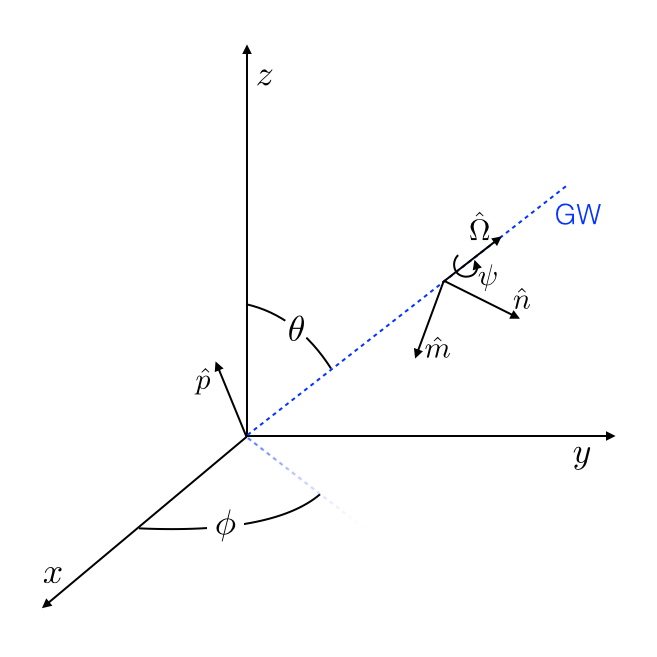
\includegraphics[width=0.8\textwidth]{Img/pulsar_position_diagram_square}
    \bicaption{脉冲星-地球系统。坐标原点选在地球。$\hat{p}$是脉冲星所在的方向。蓝色虚线代表引力波的传播方向。}{The pulsar-Earth system, as visualized with
        the Earth at the origin. The pulsar locates along $\hat{p}$ direction. The gravitational wave propagates as the
        blue dashed line.}
    \label{position_diagram}
\end{figure}
%%%%%%%%%%%%%%%%%%%%%%%%%

引力波引起的脉冲信号的红移不仅取决于脉冲星和地球系统的几何位置关系,还取决于引力波对应的度规扰动\cite{Detweiler:1979wn}。对于位于单位矢量$\hat{p}$方向(即从地球到脉冲的方向)的脉冲星,以及延$\hat{\Omega}$方向传播的引力波(见\Fig{position_diagram}),脉冲信号的红移和度规扰动的改变呈正比,即\cite{Detweiler:1979wn}
%
\beq
z(t,\hat{\Omega}) = 
\frac{1}{2}
\frac{\hat{p}^i\hat{p}^j}{1+\hat{\Omega}\cdot\hat{p}}\Delta h_{ij},
\label{tdredshift}
\eeq
其中
\beq
\Delta h_{ij}
\equiv
h_{ij}(t_{\rm e},\hat{\Omega}) - 
h_{ij}(t_{\rm p},\hat{\Omega}).
\label{delhdef}
\eeq 
上式的$t_{\rm p}$和$t_{\rm e}$分别表示脉冲信号发射的时刻和到达地球的时刻。通过对\Eq{tdredshift}的角度沿天空所有方向进行积分,可以得到总的红移
\beq
z(t) = \int_{S^2} d\hat{\Omega} \, z(t,\hat{\Omega}).
\label{zftot}
\eeq
在脉冲星探测时,我们观测到的并不是红移,而是脉冲信号的计时残差,其为红移的积分,即
\beq
r(t) = \int_0^{t} dt' \, z(t').
\label{residual}
\eeq

我们将度规扰动用平面波展开为\cite{Allen:1997ad}
\beq
h_{ij}(t,\vec{x}) = \sum_{A}
\int_{-\infty}^{\infty}df\, \int_{S^2}d\hat{\Omega}\, 
e^{i2\pi f(t-\hat{\Omega}\cdot\vec{x})}
h_A(f,\hat{\Omega})e_{ij}^A(\hat{\Omega}),
\label{pwexp}
\eeq
其中$f$是引力波的频率,$A = +, \times$表示引力波的极化,而$e_{ij}^A(\hat{\Omega})$为引力波的极化张量。利用上式的平面波分解,我们可以得到频率空间的计时残差(timing residual)为%
\e
    \tilde{r}(f,\hat{\Omega}) 
    = \frac{1}{2 \pi i f}\left(1-e^{-2\pi i f L(1+\hat{\Omega}\cdot\hat{p})}\right) 
    \sum_{A} h_A(f,\hat{\Omega}) \left ( e^A_{ij}(\hat{\Omega})
    \frac{\hat{p}^i\hat{p}^j}{2(1+\hat{\Omega}\cdot\hat{p})}\right),
    \label{fdredshift}
\q
其中$L$为脉冲星和地球的距离。极化张量的表达式为
\begin{subequations}
    \begin{align}
        \label{e_plus}
        e_{ij}^+({\hat{\Omega}}) &=  {\hat{m}}_i {\hat{m}}_j - {\hat{n}}_i {\hat{n}}_j,\\
        \label{e_cross}
        e_{ij}^{\times}({\hat{\Omega}}) &= {\hat{m}}_i {\hat{n}}_j + {\hat{n}}_i {\hat{m}}_j.
    \end{align}
\end{subequations}
\Fig{position_diagram}的各个方向为
\begin{subequations}
    \begin{align}
        \label{omega}
        {\hat{\Omega}}&= (\sin{\theta} \cos{\phi},  \sin{\theta} \sin{\phi},  
        \cos{\theta})=\hat r, \\
        \label{m}
        {\hat{m}}&=(\sin{\phi}, -\cos{\phi}, 0)=-\hat\phi, \\
        \label{n}
        {\hat{n}}&=(\cos{\theta}\cos{\phi}, \cos{\theta}\sin{\phi}, -\sin{\theta})=\hat\theta.
    \end{align}
\end{subequations}
假定随机引力波背景是各向同性的、无极化的和稳态的,应变的关联函数为\cite{Detweiler:1979wn}
\e
    \langle h_A^*(f,\hat{\Omega})h_{A'}(f',\hat{\Omega}')\rangle 
    =\frac{3H_0^2}{32\pi^3}\delta^2(\hat{\Omega},\hat{\Omega}')\delta_{AA'}
    \delta(f-f')
    |f|^{-3}\Omega_{\rm GW}(|f|).
    \label{hevom}
\q
所以脉冲星计时残差之间的关联为
\beq\label{e:rexpect}
\langle\tilde{r}_I^*(f)\tilde{r}_J(f')\rangle
= \frac{H_0^2}{16 \pi^4} \delta(f-f')|f|^{-5}
\Omega_{\rm GW}(|f|) \Gamma_{IJ},
\eeq
其中$\Gamma_{IJ}$是脉冲星$I$和脉冲星$J$之间的关联函数(即Hellings \& Downs关联系数)\cite{Hellings:1983fr}
\e\label{hd}
\Gamma_{IJ}=\frac{3}{2} \left[ \frac{1}{3} +
\frac{1-\cos\zeta_{IJ}}{2}\left[ \ln\lp\frac{1-\cos\zeta_{IJ}}{2}\rp
- \frac{1}{6} \right] \right] +\frac{1}{2}\delta_{IJ}.
\q 
上式的$\zeta_{IJ}$是脉冲星$I$和脉冲星$J$之间的角度。脉冲星计时阵列探测随机引力波背景的关键目标就是探测到\Eq{e:rexpect}所对应的关联。